% Template for Cogsci submission with R Markdown

% Stuff changed from original Markdown PLOS Template
\documentclass[10pt, letterpaper]{article}

\usepackage{cogsci}
\usepackage{pslatex}
\usepackage{float}
\usepackage{caption}

% amsmath package, useful for mathematical formulas
\usepackage{amsmath}

% amssymb package, useful for mathematical symbols
\usepackage{amssymb}

% hyperref package, useful for hyperlinks
\usepackage{hyperref}

% graphicx package, useful for including eps and pdf graphics
% include graphics with the command \includegraphics
\usepackage{graphicx}

% Sweave(-like)
\usepackage{fancyvrb}
\DefineVerbatimEnvironment{Sinput}{Verbatim}{fontshape=sl}
\DefineVerbatimEnvironment{Soutput}{Verbatim}{}
\DefineVerbatimEnvironment{Scode}{Verbatim}{fontshape=sl}
\newenvironment{Schunk}{}{}
\DefineVerbatimEnvironment{Code}{Verbatim}{}
\DefineVerbatimEnvironment{CodeInput}{Verbatim}{fontshape=sl}
\DefineVerbatimEnvironment{CodeOutput}{Verbatim}{}
\newenvironment{CodeChunk}{}{}

% cite package, to clean up citations in the main text. Do not remove.
\usepackage{apacite}

% KM added 1/4/18 to allow control of blind submission


\usepackage{color}

% Use doublespacing - comment out for single spacing
%\usepackage{setspace}
%\doublespacing


% % Text layout
% \topmargin 0.0cm
% \oddsidemargin 0.5cm
% \evensidemargin 0.5cm
% \textwidth 16cm
% \textheight 21cm

\title{Identifying the distributional sources of children's early
vocabulary}

\usepackage{booktabs}
\usepackage{longtable}
\usepackage{array}
\usepackage{multirow}
\usepackage{wrapfig}
\usepackage{float}
\usepackage{colortbl}
\usepackage{pdflscape}
\usepackage{tabu}
\usepackage{threeparttable}
\usepackage{threeparttablex}
\usepackage[normalem]{ulem}
\usepackage{makecell}
\usepackage{xcolor}

\author{{\large \bf George Kachergis* (kachergis@stanford.edu)} \\ Department of Psychology, Stanford University \\ Stanford, CA 94305 USA \AND {\large \bf Georgia Loukatou* (@stanford.edu)} \\ Department of Psychology, Stanford University \\ Stanford, CA 94305 USA \AND {\large \bf Michael C. Frank (mcfrank@stanford.edu)} \\ Department of Psychology, Stanford University \\ Stanford, CA 94305 USA}

\newlength{\cslhangindent}
\setlength{\cslhangindent}{1.5em}
\newenvironment{CSLReferences}%
  {}%
  {\par}

\begin{document}

\maketitle

\begin{abstract}
Children's early word learning is to a large extent driven by the
prevalence of words in their language environment, with words that are
spoken more often to children being learned earlier. However, children
receive language from a variety of sources, including books, television,
and movies meant for children, as well as speech and media that is meant
for adults, but overheard by children. Despite considerable similarity
of word frequency distributions from these different input sources,
there is also significant and predictable variability between them. For
example, function words are far more frequent in books than in everyday
speech, while early-learned nouns (e.g., `ball' and `mommy') are more
frequent in child-directed speech than in other sources. Children
receive a mixture of these different frequency distributions. The goal
of this paper is to better understand the shared and unique variance in
these sources of input--in both English and French--and to evaluate how
predictive these input frequencies are of children's early word
learning.

\textbf{Keywords:}
early language learning; CDI; vocabulary development; word frequency
distributions.
\end{abstract}

\hypertarget{introduction}{%
\section{Introduction}\label{introduction}}

How does speech addressed to children, heard on television, or read in
books impact the growth of children's early vocabulary? How does speech
from these sources relate to adult-directed sources of speech? And how
do these potential language sources combine with parental education to
predict young children's vocabulary growth? Children must learn words
based on ambient linguistic input, and indeed the amount of
child-directed speech a child receives predicts later vocabulary growth
(Hart \& Risley, 1995). However, children's exposure to different words
can vary greatly depending on the source -- spoken language vs.~books
vs.~media -- and the register -- child-directed vs.~adult directed -- of
the language. Moreover, the amount of input children receive from these
different input sources may vary from child to child, which may account
for some of the great variability seen in children's early vocabulary
growth (cf. Larry Fenson et al., 1994). Indeed, higher measures of input
quantity and quality have been found to relate to children's faster
vocabulary growth, and to often be related to parents' socioeconomic
status {[}SES; Rowe (2012); Hoff (2003){]}.

Input word frequency varies significantly depending on the context.
Previous studies have shown that frequency matters for children's word
learning (for a review, see Ambridge, Kidd, Rowland, \& Theakston,
2015), and have observed an association between word frequency in
children's language environments and age of acquisition (Goodman, Dale,
\& Li, 2008). For instance, word frequency in books is not the same as
frequency in conversational speech, with many function words being far
more frequent in books than in speech (Dawson, Hsiao, Wei Ming Tan,
Banerji, \& Nation, 2021; Montag, Jones, \& Smith, 2015).

Some differences between frequency distributions are intuitive:
``mommy'' is quite frequent in child-directed speech, yet not so common
in children's books, and even more rare in books meant for all ages. But
other differences are less intuitive: ``of'' is frequent in books meant
for all ages, and while still frequent in child-directed speech, it is
relatively less frequent as compared to children's books. In general,
speech -- whether directed to children or to adults -- contains
relatively fewer function words and tends to score lower on measures of
lexical diversity than books, which have a higher ratio of types (unique
words) per set of tokens {[}instances of words; Dawson, Hsiao, Wei Ming
Tan, Banerji, \& Nation (2021){]}.

In this paper, we have three primary research questions. Question 1:
First, we examine shared and unique variance in word frequency across
different sources of English and French input, ranging from children's
books and movies to child-directed speech and even comparing to
adult-directed books, movies, and speech. Because of the substantial
correlations between these different input sources, we employ principal
components analysis (PCA) for dimensionality reduction.

Question 2: Second, we investigate how well these components predict
English- and French-learning children's early word learning, using
aggregate MacArthur-Bates Communicative Development Inventories (CDI)
data from Wordbank (Frank, Braginsky, Yurovsky, \& Marchman, 2017). CDIs
are parent report forms for children's early vocabulary, and they have
proven to be reliable and valid indicators of child's language (Larry
Fenson et al., 1994). Critically, CDI forms provide details about the
individual words that children produce. These data allow us to
investigate the role of different frequency sources using the Age of
Acquisition (AoA) prediction paradigm, in which we use regression models
to predict each CDI item's mean Age of Acquisition (AoA) -- the mean age
(in months) at which 50\% of children are expected to know a given word
(Braginsky, Yurovsky, Marchman, \& Frank, 2019; Goodman, Dale, \& Li,
2008).

Question 3: Third, we examine how well different input sources predict
SES differences in word learning for English-learning children. We index
SES using maternal education, a common proxy measure. Young children
from higher-SES households tend to have larger vocabulary (Fernald,
Marchman, \& Weisleder, 2013) and parents with higher-SES tend to report
reading more to their young children than parents with lower SES.

Together, the answers to these questions provide insight into whether
word frequency acts as a single factor in vocabulary learning, or
whether different sources and registers have distinguishable effects.

\hypertarget{method}{%
\section{Method}\label{method}}

\hypertarget{datasets}{%
\subsection{Datasets}\label{datasets}}

Corpora from different sources are used to identify shared and distinct
variance in frequencies. These corpora vary widely in size due to data
accessibility; several were created for the current study and are
available in our GitHub repository.

\hypertarget{child-directed-speech-chs.}{%
\subsubsection{Child-directed Speech
(ChS).}\label{child-directed-speech-chs.}}

Utterances of ChS were extracted from the CHILDES corpus (MacWhinney,
2000), a collection of transcripts of interactions between caregivers
and children of ages ranging from 0 to 12 years (\(M=2.9\) years). After
cleaning, the CHILDES English corpus yielded 5521000 tokens across 38779
word types. The French ChS yielded 3102000 tokens across 13016 word
types.

\hypertarget{child-directed-books-chb.}{%
\subsubsection{Child-directed books
(ChB).}\label{child-directed-books-chb.}}

We used a sample of 98 English children's books from Project Gutenberg's
open-source database, previously used in machine learning research on
language comprehension (Hill, Bordes, Chopra, \& Weston, 2015). The
books were published between 1820 and 1922, but include well-known
titles as \emph{The Legend of Sleepy Hollow}. We also used 130 popular
French children stories accessible in parenting websites
(\url{https://fr.hellokids.com/}) and 10 French children books from
Project Gutenberg. After cleaning, the English ChB corpus totals 4673000
tokens across 42444 word types, and the French ChB totals 1298000 tokens
across 17990 word types.

\hypertarget{child-directed-media-chm.}{%
\subsubsection{Child-directed Media
(ChM).}\label{child-directed-media-chm.}}

Transcripts were extracted from English television shows (e.g., from PBS
Kids and Nickelodeon) and movies (e.g., \emph{Beauty and the Beast}),
including 1,078 movies and 4,309 TV episodes taken from Charlesworth,
Yang, Mann, Kurdi, \& Banaji (2021) (available here:
\url{https://osf.io/kqux5/}. Openly accessible transcripts
(\url{https://www.subsynchro.com/}) were also extracted from 100 French
films directed to children. After cleaning, the English ChM totals
6723850 tokens across 80082 word types. The French ChM totals 842000
tokens across 14937 word types.

\hypertarget{adult-directed-speech-ads.}{%
\subsubsection{Adult-directed Speech
(AdS).}\label{adult-directed-speech-ads.}}

English AdS was obtained from the Switchboard-1 Telephone Speech Corpus
(Godfrey \& Holliman, 1993), a corpus of transcripts from approximately
2,400 dyadic telephone conversations. After cleaning, the English AdS
yielded 3104000 tokens across 27479 word types. French AdS was obtained
from the TCOF corpus (André \& Canut, 2010), the CLAPI corpus (Balthasar
\& Bert, 2005) and the CFPP corpus (Branca-Rosoff, Fleury, Lefeuvre, \&
Pires, 2012). The French AdS yielded 1466000 tokens across 14486 word
types.

\hypertarget{adult-directed-books-adb.}{%
\subsubsection{Adult-directed Books
(AdB).}\label{adult-directed-books-adb.}}

The English AdB corpus is taken from a sample of 1,000 Project Gutenberg
books tokens randomly selected by Charlesworth, Yang, Mann, Kurdi, \&
Banaji (2021), totaling 40252700 tokens across 147937 word types. The
French AdB is comprised of books taken from the 1999 Association de
Bibliophiles Universels, an open-source database of french books. After
cleaning, it yielded 2288000 tokens across 30615 word types.

\hypertarget{adult-directed-media-adm.}{%
\subsubsection{Adult-directed Media
(AdM).}\label{adult-directed-media-adm.}}

The English AdM is comprised of 6060000 tokens across 60626 word types
compiled by Charlesworth, Yang, Mann, Kurdi, \& Banaji (2021) from
online transcripts of movies and TV shows dating from the 1960s (e.g.,
\emph{Doctor Who}) through the present (e.g., \emph{Breaking Bad}). The
French AdM corpus is comprised of 766000 tokens across 15662 word types,
after cleaning openly accessible movie subtitles
(\url{https://www.subsynchro.com/}) from 100 films.

\hypertarget{age-of-acquisition-data}{%
\subsubsection{Age of Acquisition data}\label{age-of-acquisition-data}}

Children's early word learning data was drawn from the CDIs (L. Fenson
et al., 2007), aggregated in the Wordbank database (Frank, Braginsky,
Yurovsky, \& Marchman, 2017) (data from 5520 children aged 16-30 months
for the American English CDI: Words \& Sentences (WS) form, and 641
children for the French French CDI:WS form). Age of acquisition
estimates were calculated via the wordbankr package. We computed the
proportion of children at each age who were reported to produce each
word on the CDI forms completed by parents. We then fit a curve to these
proportions using a logistic regression model and determined when the
predicted acquisition curve crossed 0.5 (when at least 50\% of children
produce the word) .

\hypertarget{merging-the-corpora}{%
\subsection{Merging the Corpora}\label{merging-the-corpora}}

We focus our analysis on the 670 words from the English CDI and 632
words from the French CDI that were present in at least one of the
corpora. For French, because of the presence of more complex morphology,
CDI words were matched to related words in corpora via a stemmer. All
word frequencies were normalized to number of tokens per million (TPM).
For any CDI words that failed to appear in a given corpus, we replaced
the missing word's frequency with a normalized count of 10 TPM, or the
minimum normalized frequency for that distribution, whichever was
smaller.

\hypertarget{results}{%
\section{Results}\label{results}}

\hypertarget{cross-corpus-frequency-correlations-q1}{%
\subsection{Cross-corpus Frequency Correlations
(Q1)}\label{cross-corpus-frequency-correlations-q1}}

\begin{CodeChunk}
\begin{figure}[t]

{\centering 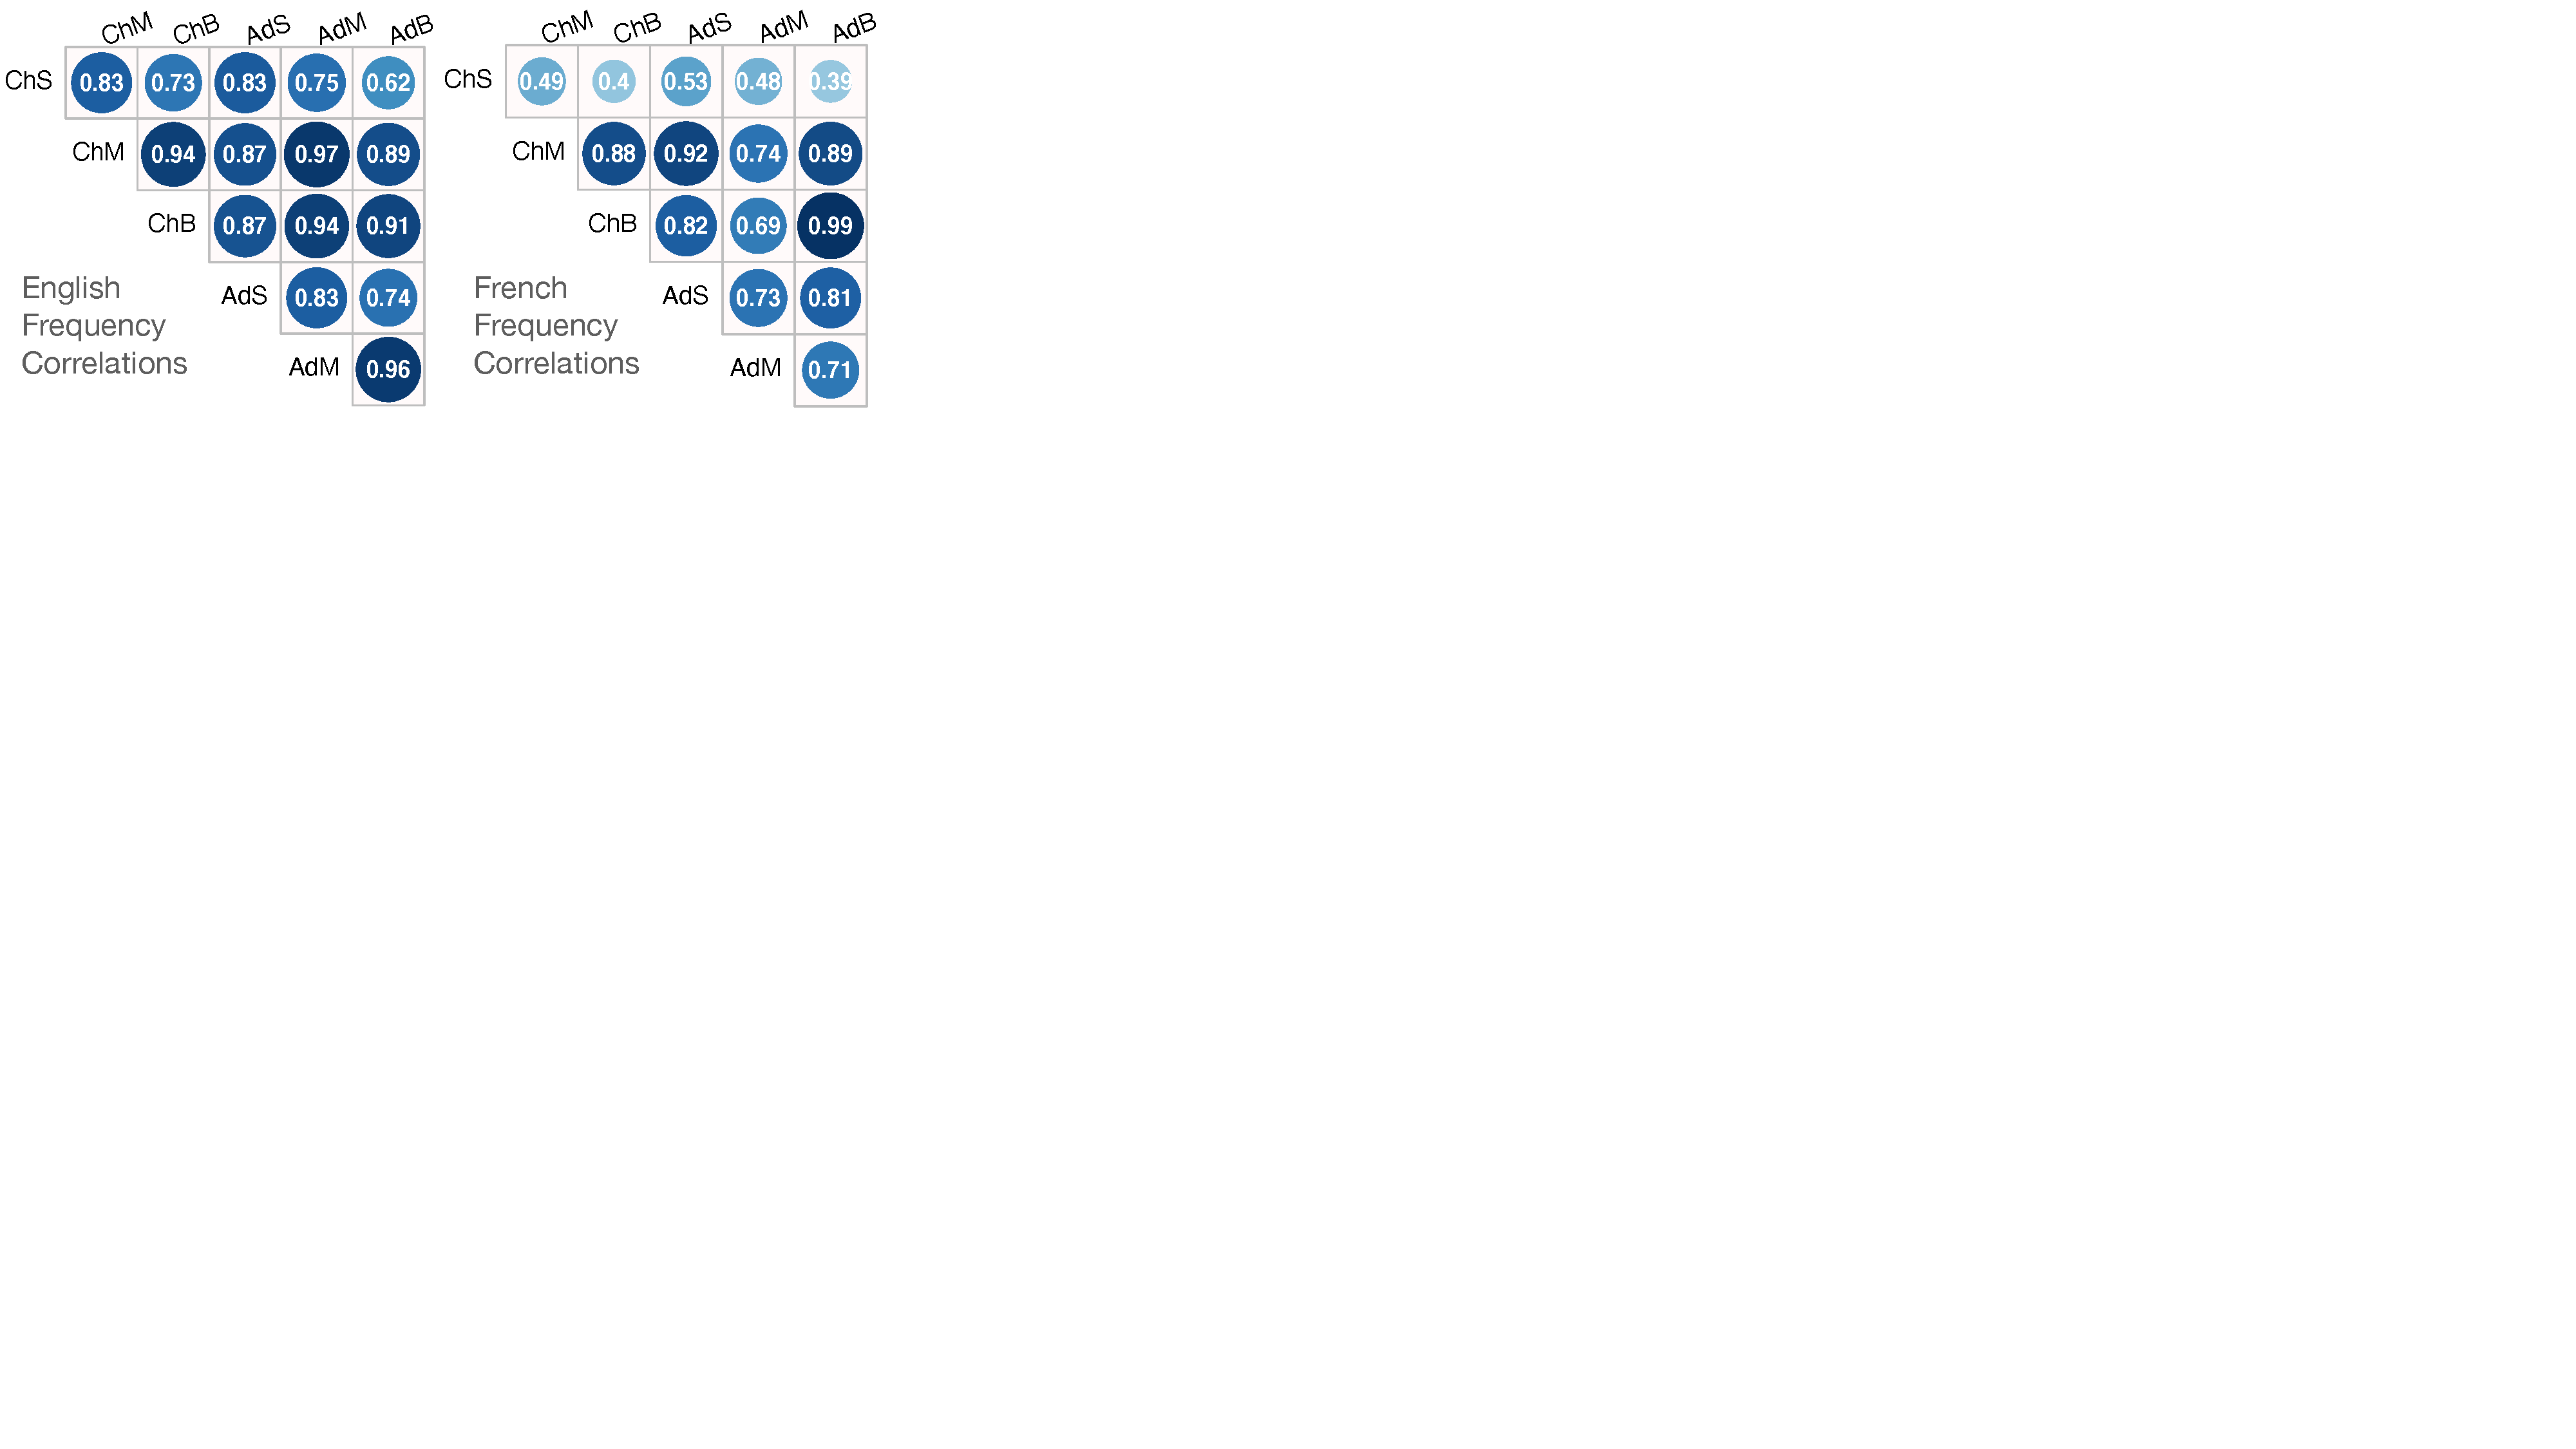
\includegraphics[width=\linewidth]{figs/corpus_freq_cors_hor} 

}

\caption[Word frequency correlations between different corpus sources for the matched CDI words in English (left) and French (right)]{Word frequency correlations between different corpus sources for the matched CDI words in English (left) and French (right).}\label{fig:fig1}
\end{figure}
\end{CodeChunk}

Figure 1 shows the word frequency correlations between different corpus
sources ({[}Adult- vs.~Child-directed{]} x {[}Speech, Books, Media{]})
for the matched CDI words (left: English, right: French).
Unsurprisingly, there were strong correlations across these different
corpora, but correlations were stronger within register and within
source for both English and French.

We thus turned to PCA to disentangle these correlated distributions and
to understand their relationship. PCA allows us to project word
frequencies into a space in which the first dimension captures the
shared variance between frequencies from different sources and
registers, and subsequent dimensions capture other consistent sources of
variation. Since the logarithm of frequency is typically used as a
psycholinguistic predictor in previous studies (Braginsky, Yurovsky,
Marchman, \& Frank, 2019; Goodman, Dale, \& Li, 2008), we perform our
PCA over log frequencies.

Table 1 provides qualitative descriptions of the principal components
(PC1-PC6) for each language. The eigenvectors of the PCs in relation to
the original six frequency distributions are summarized for English in
Table 2, and for French in Table 3, along with the proportion of
variance (PVar) explained by each component. PC1 already explains the
bulk of the variance (89\% for English and 90.1\% for French); and
PC2-PC4 each only capture an additional 2-4\% of the variance for both
languages. Note that the signs of eigenvectors in PCA are arbitrary, and
so for ease of interpretation, whever possible we describe findings in
the positive direction.

The first PC is similar for both English and French, and captures shared
variance between all frequency sources and registers, representing words
that are high or low frequency across them. This means that frequency
distributions are largely similar across sources and registers. The
second PC for English mostly captures child-directed speech,
differentiating it from ll the other registers, whereas for French it
captures book language, differentiating it from speech. PC2 explains
3.8\% of variance for English and 4.4\% of variance for French.
Adult-directed speech is captured in English as the third PC (3.2\% of
variance), whereas the difference between child-directed and
adult-directed speech is captured in French as the third PC (2.6\% of
variance). The additional PCs capture differences between media and book
or speech, as well as differences between media registers
(child-directed vs adult-directed) for both languages.

In summary, the PCs align surprisingly well with particular dimensions
of the English frequency distributions: PC1 with overall frequency, PC2
with child-directed speech, PC3 with adult-directed speech, PC4 with
media vs.~books, PC5 with child-directed books vs.~speech, and PC6 with
adult- vs.~child-directed media. For French, we observe a similar
pattern of findings. A difference lies on PC2; whereas it captures
register differences, especially for child-directed speech comparing it
to all other sources in English; it captures source differences in
French, distinguishing book language from speech.

\begin{CodeChunk}



\begin{table}[tbp]

\begin{center}
\begin{threeparttable}

\caption{\label{tab:table1}Descriptions of English and French PCs based on their order of importance, as well as the words with the highest and lowest values within each PC. CDS stands for child-directed speech. ADS stands for adult-directed speech. CDB stands for child-directed books. CDM stands for child-directed media. ADM stands for adult-directed speech. ADB stands for adult-directed books. EN stands for English and FR stands for French. 'le' = 'the', 'ça' = 'this', 'lequel' = 'which', 'salut' = 'hi', 'madeleine' = 'small cake', 'grand-mère' = 'grandmother', 'doigt de pied' = 'toe', 'sombre' = 'dark', 'parce que' = 'because', 'carottes' = 'carrots'.}

\begin{tabular}{lllll}
\toprule
Lang & \multicolumn{1}{c}{PC} & \multicolumn{1}{c}{Description} & \multicolumn{1}{c}{Highest} & \multicolumn{1}{c}{Lowest}\\
\midrule
EN & 1 & overall freq & play dough & the\\
EN & 2 & CDS & don't & tissue\\
EN & 3 & ADS & don't & gotta\\
EN & 4 & Media/Book & camera & was\\
EN & 5 & CDS/CDB & grrr & mommy\\
EN & 6 & CDM/ADM & beans & don't\\
FR & 1 & overall freq & doigt de pied & le\\
FR & 2 & Book/Speech & sombre & ça\\
FR & 3 & CDS/ADS & élephant & lequel\\
FR & 4 & Media/Speech & parce que & salut\\
FR & 5 & CDM/ADM & grand-mère & madeleine\\
FR & 6 & CDB/ADB & carottes & grand-mère\\
\bottomrule
\end{tabular}

\end{threeparttable}
\end{center}

\end{table}


\end{CodeChunk}

\begin{CodeChunk}
\begin{table}

\caption{\label{tab:pca-en-table}English PC rotations and the proportion of variance (PVar) for each PC. The lowest values have black cells, and the highest values have orange cells.}
\centering
\begin{tabular}[t]{>{}l>{}r>{}r>{}r>{}r>{}r>{}r}
\toprule
  & PC1 & PC2 & PC3 & PC4 & PC5 & PC6\\
\midrule
\cellcolor{white}{\textcolor{black}{ChM}} & \cellcolor[HTML]{1B1043}{\textcolor{white}{\em{-0.31}}} & \cellcolor[HTML]{A02F7F}{\textcolor{white}{0.15}} & \cellcolor[HTML]{000004}{\textcolor{white}{\textbf{-0.34}}} & \cellcolor[HTML]{FB835F}{\textcolor{white}{0.40}} & \cellcolor[HTML]{E44F64}{\textcolor{white}{0.28}} & \cellcolor[HTML]{FE9F6D}{\textcolor{white}{\textbf{0.73}}}\\
\cellcolor{white}{\textcolor{black}{ChB}} & \cellcolor[HTML]{150E37}{\textcolor{white}{\em{-0.34}}} & \cellcolor[HTML]{BB3978}{\textcolor{white}{0.25}} & \cellcolor[HTML]{020109}{\textcolor{white}{-0.32}} & \cellcolor[HTML]{000004}{\textcolor{white}{-0.63}} & \cellcolor[HTML]{FE9F6D}{\textcolor{white}{\textbf{0.53}}} & \cellcolor[HTML]{3D0F71}{\textcolor{white}{-0.21}}\\
\cellcolor{white}{\textcolor{black}{ChS}} & \cellcolor[HTML]{251254}{\textcolor{white}{\em{-0.26}}} & \cellcolor[HTML]{FE9F6D}{\textcolor{white}{\textbf{0.65}}} & \cellcolor[HTML]{030312}{\textcolor{white}{-0.30}} & \cellcolor[HTML]{C53C74}{\textcolor{white}{0.12}} & \cellcolor[HTML]{000004}{\textcolor{white}{\textbf{-0.60}}} & \cellcolor[HTML]{38106C}{\textcolor{white}{-0.22}}\\
\cellcolor{white}{\textcolor{black}{AdM}} & \cellcolor[HTML]{030310}{\textcolor{white}{\em{-0.47}}} & \cellcolor[HTML]{02020B}{\textcolor{white}{-0.45}} & \cellcolor[HTML]{0D0A29}{\textcolor{white}{-0.24}} & \cellcolor[HTML]{FE9F6D}{\textcolor{white}{\textbf{0.48}}} & \cellcolor[HTML]{BC3978}{\textcolor{white}{0.13}} & \cellcolor[HTML]{000004}{\textcolor{white}{\textbf{-0.53}}}\\
\cellcolor{white}{\textcolor{black}{AdB}} & \cellcolor[HTML]{020109}{\textcolor{white}{\em{-0.49}}} & \cellcolor[HTML]{000004}{\textcolor{white}{\textbf{-0.47}}} & \cellcolor[HTML]{491078}{\textcolor{white}{-0.01}} & \cellcolor[HTML]{21114E}{\textcolor{white}{-0.44}} & \cellcolor[HTML]{0C0927}{\textcolor{white}{-0.50}} & \cellcolor[HTML]{C63C73}{\textcolor{white}{0.32}}\\
\addlinespace
\cellcolor{white}{\textcolor{black}{AdS}} & \cellcolor[HTML]{000004}{\textcolor{white}{\em{-0.52}}} & \cellcolor[HTML]{C23B75}{\textcolor{white}{0.27}} & \cellcolor[HTML]{FE9F6D}{\textcolor{white}{\textbf{0.79}}} & \cellcolor[HTML]{C13A75}{\textcolor{white}{0.10}} & \cellcolor[HTML]{C03A77}{\textcolor{white}{0.14}} & \cellcolor[HTML]{721F81}{\textcolor{white}{-0.01}}\\
\cellcolor{white}{\textcolor{black}{PVar}} & \cellcolor{white}{\textcolor{black}{0.89}} & \cellcolor{white}{\textcolor{black}{0.04}} & \cellcolor{white}{\textcolor{black}{0.03}} & \cellcolor{white}{\textcolor{black}{0.02}} & \cellcolor{white}{\textcolor{black}{0.01}} & \cellcolor{white}{\textcolor{black}{0.01}}\\
\bottomrule
\end{tabular}
\end{table}

\end{CodeChunk}

\begin{CodeChunk}
\begin{table}

\caption{\label{tab:pca-fr-table}French principal component rotations.}
\centering
\begin{tabular}[t]{>{}l>{}r>{}r>{}r>{}r>{}r>{}r}
\toprule
  & PC1 & PC2 & PC3 & PC4 & PC5 & PC6\\
\midrule
\cellcolor{white}{\textcolor{black}{ChM}} & \cellcolor[HTML]{010107}{\textcolor{white}{\em{-0.41}}} & \cellcolor[HTML]{6C1D81}{\textcolor{white}{-0.09}} & \cellcolor[HTML]{812581}{\textcolor{white}{0.05}} & \cellcolor[HTML]{000004}{\textcolor{white}{\textbf{-0.65}}} & \cellcolor[HTML]{FE9F6D}{\textcolor{white}{\textbf{0.56}}} & \cellcolor[HTML]{DF4968}{\textcolor{white}{0.31}}\\
\cellcolor{white}{\textcolor{black}{ChB}} & \cellcolor[HTML]{010105}{\textcolor{white}{\em{-0.41}}} & \cellcolor[HTML]{FE9F6D}{\textcolor{white}{\textbf{0.54}}} & \cellcolor[HTML]{AB337C}{\textcolor{white}{0.21}} & \cellcolor[HTML]{BD3977}{\textcolor{white}{0.13}} & \cellcolor[HTML]{DF4968}{\textcolor{white}{0.26}} & \cellcolor[HTML]{000004}{\textcolor{white}{\textbf{-0.64}}}\\
\cellcolor{white}{\textcolor{black}{ChS}} & \cellcolor[HTML]{050415}{\textcolor{white}{\em{-0.36}}} & \cellcolor[HTML]{000004}{\textcolor{white}{\textbf{-0.51}}} & \cellcolor[HTML]{FE9F6D}{\textcolor{white}{\textbf{0.73}}} & \cellcolor[HTML]{D6456C}{\textcolor{white}{0.22}} & \cellcolor[HTML]{681C81}{\textcolor{white}{-0.16}} & \cellcolor[HTML]{922B80}{\textcolor{white}{0.02}}\\
\cellcolor{white}{\textcolor{black}{AdM}} & \cellcolor[HTML]{000004}{\textcolor{white}{\em{-0.42}}} & \cellcolor[HTML]{4E117B}{\textcolor{white}{-0.19}} & \cellcolor[HTML]{1F114A}{\textcolor{white}{-0.34}} & \cellcolor[HTML]{261256}{\textcolor{white}{-0.42}} & \cellcolor[HTML]{000004}{\textcolor{white}{\textbf{-0.62}}} & \cellcolor[HTML]{38106C}{\textcolor{white}{-0.34}}\\
\cellcolor{white}{\textcolor{black}{AdB}} & \cellcolor[HTML]{010107}{\textcolor{white}{\em{-0.41}}} & \cellcolor[HTML]{FD9C6B}{\textcolor{white}{\textbf{0.54}}} & \cellcolor[HTML]{7C2382}{\textcolor{white}{0.02}} & \cellcolor[HTML]{CC3F71}{\textcolor{white}{0.18}} & \cellcolor[HTML]{321066}{\textcolor{white}{-0.36}} & \cellcolor[HTML]{FE9F6D}{\textcolor{white}{\textbf{0.62}}}\\
\addlinespace
\cellcolor{white}{\textcolor{black}{AdS}} & \cellcolor[HTML]{000004}{\textcolor{white}{\em{-0.42}}} & \cellcolor[HTML]{1E1149}{\textcolor{white}{-0.34}} & \cellcolor[HTML]{000004}{\textcolor{white}{\textbf{-0.55}}} & \cellcolor[HTML]{FE9F6D}{\textcolor{white}{\textbf{0.55}}} & \cellcolor[HTML]{E55064}{\textcolor{white}{0.30}} & \cellcolor[HTML]{9A2D80}{\textcolor{white}{0.04}}\\
\cellcolor{white}{\textcolor{black}{PVar}} & \cellcolor{white}{\textcolor{black}{0.90}} & \cellcolor{white}{\textcolor{black}{0.04}} & \cellcolor{white}{\textcolor{black}{0.03}} & \cellcolor{white}{\textcolor{black}{0.02}} & \cellcolor{white}{\textcolor{black}{0.01}} & \cellcolor{white}{\textcolor{black}{0.00}}\\
\bottomrule
\end{tabular}
\end{table}

\end{CodeChunk}

\hypertarget{pca-based-age-of-acquisition-regression-q2}{%
\subsection{PCA-based Age of Acquisition Regression
(Q2)}\label{pca-based-age-of-acquisition-regression-q2}}

Next, we turned to our second question: how well different frequency
distributions predict English- and French-learning children's early word
learning. Our approach was to fit a linear regression model predicting
each CDI word's mean AoA, following previous work (Braginsky, Yurovsky,
Marchman, \& Frank, 2019; Goodman, Dale, \& Li, 2008).

Multicollinearity makes it unwise to include multiple raw frequency
distributions in a regression, however, as the results will be unstable.
We verified that this situation was the case by running a regression
predicting AoA with the logarithm of word frequency from each of the six
distributions as a predictor. The Variance Inflation Factor (VIF)
estimates the inflation of the variance of a regression coefficient when
there is correlation between predictors (Dodge, 2008). The higher the
VIF for a predictor, the less reliable the regression results are when
that predictor is included. The VIF for every distribution was \(>>1\)
(and many \(>5\)), indicating that these variables show strong
multicollinearity which may compromise the reliability of the regression
results. We thus used the CDI items' PCA loadings in lieu of the
frequency distributions to predict AoA.

Given that past research has found that lexical class strongly modulates
influences of word frequency, we included the interaction of lexical
class (LC) with PC1 - PC6 in our regression. We also included the number
of letters as a predictor (Nletters) to help control for the overall
difficulty of producing each word {[}within each language, this
predictor is extremely correlated with the number of phonemes and serves
as a good proxy for production complexity;
(\textbf{braginsky2018consistency?}){]}. To determine if the inclusion
of all PCs was justified, we ran a series of ANOVAs building up from PC1
to PC6 -- in decreasing order of the variance they accounted for in the
PCA\footnote{The R syntax for the sequence of regressions was
  \texttt{AoA}\(\sim\)\texttt{PC1*LC},
  \texttt{AoA}\(\sim\)\texttt{(PC1+PC2)*LC}, \ldots,
  \texttt{AoA}\(\sim\)\texttt{(PC1+PC2+PC3+PC4+PC5+PC6)*LC}, with noun
  as the baseline LC.}. For English, the more complex model was always
significantly preferred, including up to the inclusion of PC6
(\(R^2 = .58\)). For French, the model which only included PC1 and PC2
as predictors was significantly preferred, even though the french model
explained less variation of the dependent value overall (\(R^2 = .06\)).
Figure 2 shows the coefficient estimates with p\textless0.05 for both
languages.

For English, PC1, PC2, PC3, PC4 and PC5 significantly predict the age of
acquisition. Overall frequency (PC1) is a predictor; words which are
frequent in general are learned earlier than less frequent words (recall
that eigenvectors on PC1 are negative and so a positive coefficient
indicates greater frequency predicts earlier learning). Child-directed
speech (PC2) is a predictor; words which are frequent in this register
are learned substantially earlier (more so than for general frequency).
On the contrary, for the adult-directed speech predictor (PC3), frequent
words are learned later.\\
Word frequency in media distinguished from words in books is a predictor
(PC4); words which are frequent in media tend to be learned earlier on.
Word frequency in child-directed speech as distinguished from words in
child-directed books is also a predictor (PC5), with earlier acquisition
predicted for more speechy/less booky words. We also observe that
overall frequency (PC1) interacts with lexical class, verbs, function
words and adjectives being learned later than nouns. PC2 interacts with
verbs, which are learned later than nouns. PC3 and PC6 each interacted
with function words, which are learned later than nouns.

For French, PC2 significantly predicts the age of acquisition, implying
the importance of both speech and book sources in explaining variation.
In general, the PC1 coefficient direction indicates that frequent words
are learned earlier than less frequent words, but it is not a
significant predictor in this regression. This could be attributed to
PC1 being explained away by PC2, or it is an artifact of the data
e.g.~some lexical category being more represented than others). PC1
interacts significantly with function words. Verbs are also a
significant predictor. In both languages, there is no significant effect
of word length.

\begin{CodeChunk}
\begin{figure}[H]

{\centering 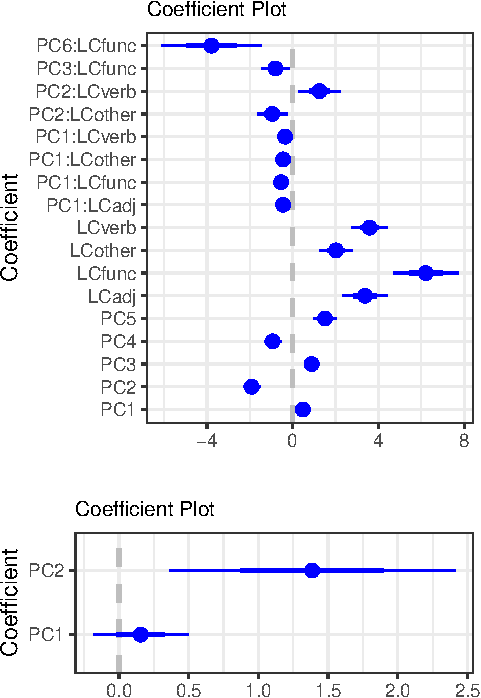
\includegraphics{figs/unnamed-chunk-8-1} 

}

\caption[Significant regression coefficients for predicting CDI AoAs with PCs and lexical class for English (top) and French (bottom)]{Significant regression coefficients for predicting CDI AoAs with PCs and lexical class for English (top) and French (bottom). 'func' stands for function words, 'other' stands for words refering to games, routines and people. 'adj' stands for 'adjective'. }\label{fig:unnamed-chunk-8}
\end{figure}
\end{CodeChunk}

To sum up, in both languages, we observe that the predictive value of
word frequency was especially high for words that are highly frequent in
child directed speech However, for English, the difference across
registers (difficulty of adult-directed versus child-directed) appears
more important. For French, the difference and difficulty of text,
independent of register, appears more important.

\hypertarget{principal-components-and-maternal-education-q3}{%
\subsection{Principal components and maternal education
(Q3)}\label{principal-components-and-maternal-education-q3}}

Previous findings relate SES status to book reading (Shen \& Del Tufo,
2022), which is in turn related to better language skills (Bus, Van
Ijzendoorn, \& Pellegrini, 1995). These findings suggest that the
vocabulary composition of children whose mothers are more
highly-educated (a proxy for household SES) may be better predicted by
the word frequencies seen in child-directed books, rather than those
from child-directed speech. To test this idea, we fit a series of
exploratory logistic regressions successively adding the PCs to predict
the number of children in Wordbank who produce or don't produce each
item. Due to lack of maternal education data for French data, we focus
on American English-learning children. We included interactions of
mother's education and children's age with each included PC;
interactions of this type indicate that a particular type of register or
source might be more important to acquisition for one SES group or
another.

American English data from Wordbank contained 2,776 CDI:WS
administrations with mother's education dichotomously coded (N=1160 with
at most some college education; N=1616 with a college degree or more).
The series of ANOVAs indicated that PC1 through PC5 significantly
improved the model fits, but that adding PC6 was not justified. Thus, we
analyzed the model that included the first five PCs.

This model showed significant main effects of age, mother's education,
and all five PCs (all \(p<.001\)). Faster learning was predicted for
words with higher values on PC1 (overall frequency; \(\beta=.10\)), PC2
(child-directed speech; \(\beta=.45\)), or PC4 ( \(\beta=.28\)). Slower
learning was predicted for words with higher values on PC3
(\(\beta=-.34\)) or PC5 (\(\beta=-.49\)).

There was a significant positive interaction of age with mother's
education (\(\beta=.06\), \(p<.001\)), shown in Figure 3. There were
also significant interactions of age and all five PCs, although the
coefficients were all of a small magnitude (\(\beta\)s \textless{} .01).
Only PC1 and PC5 interacted significantly with mother's education. Shown
in Figure 3, children of higher-educated mothers were more likely to
know words that were higher on PC1 (overall frequency; \(\beta = .03\),
\(p<.001\)), while they were less likely to know words that were high on
PC5 (\(\beta = -.09\), \(p=.01\)). Words more frequent in child-directed
speech are high on PC5, while words that are more often in
child-directed books are low on PC5, meaning that this interaction
indicates children with higher-educated mothers are more likely to learn
booky (rather than speechy) words.

There was one significant 3-way interaction of age, mother's education,
and PC1, with a small magnitude negative coefficient (\(\beta=-.001\)).

\begin{CodeChunk}
\begin{figure}[H]

{\centering 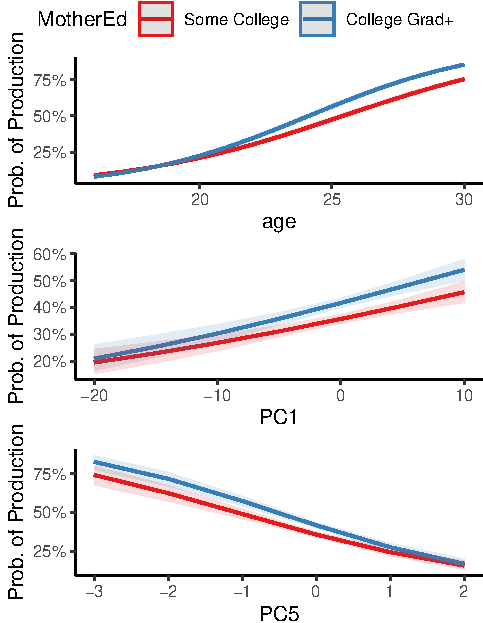
\includegraphics{figs/unnamed-chunk-10-1} 

}

\caption[Predicted effects on the probability of English-speaking children producing CDI:WS words based level of maternal education]{Predicted effects on the probability of English-speaking children producing CDI:WS words based level of maternal education. A significant positive interaction with age (top) shows an increasing effect of maternal education as children age. A significant positive interaction with PC1 (middle) shows that words with higher overall frequency are produced more by children with more educated mothers. Finally, a negative interaction with PC5 shows that children with more educated mothers are likely to produce words more representative of child-directed books, rather than child-directed speech.}\label{fig:unnamed-chunk-10}
\end{figure}
\end{CodeChunk}

\hypertarget{discussion}{%
\section{Discussion}\label{discussion}}

We set out to investigate the sources of linguistic input and registers
that children may experience, using word frequency distributions
garnered from child-directed and adult-directed corpora of speech,
books, and media (TV and movies). We found the principal components
(PCs) of these distributions, and described how these PCs capture
variation both in adult- vs.~child-directedness, as well as between
modalities (e.g., books and speech).

Our findings show that PC1 explains 90\% of the variance in frequency
distributions for both languages. This means that most frequency is
shared by all the different sources and registers in our study, and is
thus accounted for by this one component. In spite of this, the
remaining prinicipal components in both languages picked up on
consistent differences in both register and source. In English,
child-directed speech captures a large part of the variance as a second
principal component, which shows that CDI word frequencies actually
differ a lot compared to all other sources. In French, in contrast,
child-directed speech loaded strongly on the third principal component,
while the second component picked up on bookish words (both child- and
adult-directed) -- a distinction captured in PC4 for English.

Multiple components are predictive of children's age of acquisition of
words from the CDI in English. Child-directed speech, adult-directed
speech, but also books and media are all relevant in predicting age of
acquisition. It is somewhat surprising that even sources of input that
young children rarely encounter (e.g., adult-directed books) contribute
significantly to predicting variation in children's early word learning,
and this suggests that children's environmental exposure to different
language sources, even when these include books or even media, could
impact their word learning trajectory.

In French, the component diversifying books and speech captures a large
part of the variance as a second principal component, and is the most
relevant one in predicting age of acquisition. This finding underlines
the importance of the speech and text sources independent of register.
On the contrary, the difference between child-directed and
adult-directed registers is not as pronounced as in our English data. We
speculate that the French word frequencies tested here do not differ
that much across registers and instead vary more between spoken and
written sources.

We also used English Wordbank data to examine how well the frequency
components combine with mother's education -- a measure of SES that has
been found in the past to be positively related to early word learning,
and to more child-directed reading -- to predict children's early word
learning. This analysis revealed significant contributions of the first
five PCs, as well as interactions of mother's education with PC1
(overall frequency) and PC5 (child-directed speech vs.~books) -- but
without any significant interaction of PC2 (child-directed speech), nor
PC3 (adult-directed speech), nor of the media component (PC4). This
finding suggests that the early language advantage shown by children of
more highly-educated mothers (and thus in higher-SES households; cf.
Hoff, 2003) may in part be due to greater amounts of shared reading
time.

This last finding is especially interesting because it suggests the
specific role of literacy practices in affecting vocabulary growth. A
target for future research is to predict individual children's learning
of particular words using these principal components, in combination
with parent-reported measures of how much time their child spends daily
receiving input from each of the input sources ({[}adult-
vs.~child-directed{]} x {[}books, media, and speech{]}).

This research has a number of limitations that point the way to future
work. First, our study is an observational linkage between frequencies
as estimated from one set of materials and acquisition trajectories from
wholly different children. We expect that frequencies represent
estimates of an average experience by a member of a particular
linguistic or cultural group, but they are certainly biased by their
specific source. Further, corpus sizes were used to represent the
sources for each language. Differences could also be partly attributed
to this e.g., the French corpora were composed of several smaller ones,
due to the lack of large accessible corpora, and had slightly different
makeup, e.g.~small stories in French vs.~large books in English.
Finally, although we made an effort to examine two languages, French and
English represent only a tiny subset of the broader set of linguistic
environments in which children acquire their vocabulary.

In sum, by better understanding the similarity and differences between
word frequencies children experience in different contexts, future
research in this vein holds the promise to predict individual
differences in children's early word learning on the basis of their
daily routines.

\hypertarget{acknowledgements}{%
\section{Acknowledgements}\label{acknowledgements}}

{[}Redacted for anonymous review.{]}

\hypertarget{references}{%
\section{References}\label{references}}

\setlength{\parindent}{-0.1in} 
\setlength{\leftskip}{0.125in}

\noindent

\hypertarget{refs}{}
\begin{CSLReferences}{1}{0}
\leavevmode\hypertarget{ref-ambridge2015ubiquity}{}%
Ambridge, B., Kidd, E., Rowland, C. F., \& Theakston, A. L. (2015). The
ubiquity of frequency effects in first language acquisition.
\emph{Journal of Child Language}, \emph{42}(2), 239--273.

\leavevmode\hypertarget{ref-andre2010mise}{}%
André, V., \& Canut, E. (2010). Mise {à} disposition de corpus oraux
interactifs: Le projet TCOF (traitement de corpus oraux en fran{ç}ais).
\emph{Pratiques. Linguistique, Litt{é}rature, Didactique}, (147-148),
35--51.

\leavevmode\hypertarget{ref-balthasar2005plateforme}{}%
Balthasar, L., \& Bert, M. (2005). La plateforme corpus de langues
parl{é}es en interaction(CLAPI). Historique, {é}tat des lieux,
perspectives. \emph{Lidil. Revue de Linguistique Et de Didactique Des
Langues}, (31), 13--33.

\leavevmode\hypertarget{ref-braginsky2019consistency}{}%
Braginsky, M., Yurovsky, D., Marchman, V. A., \& Frank, M. C. (2019).
Consistency and variability in children's word learning across
languages. \emph{Open Mind}, \emph{3}, 52--67.

\leavevmode\hypertarget{ref-branca2012discours}{}%
Branca-Rosoff, S., Fleury, S., Lefeuvre, F., \& Pires, M. (2012).
Discours sur la ville. Pr{é}sentation du corpus de fran{ç}ais parl{é}
parisien des ann{é}es 2000 (CFPP2000). \emph{Article En Ligne,
Http://Cfpp2000. Univparis3. Fr/Articles. Html}.

\leavevmode\hypertarget{ref-bus1995joint}{}%
Bus, A. G., Van Ijzendoorn, M. H., \& Pellegrini, A. D. (1995). Joint
book reading makes for success in learning to read: A meta-analysis on
intergenerational transmission of literacy. \emph{Review of Educational
Research}, \emph{65}(1), 1--21.

\leavevmode\hypertarget{ref-charlesworth2021gender}{}%
Charlesworth, T. E., Yang, V., Mann, T. C., Kurdi, B., \& Banaji, M. R.
(2021). Gender stereotypes in natural language: Word embeddings show
robust consistency across child and adult language corpora of more than
65 million words. \emph{Psychological Science}, \emph{32}(2), 218--240.

\leavevmode\hypertarget{ref-dawson2021features}{}%
Dawson, N., Hsiao, Y., Wei Ming Tan, A., Banerji, N., \& Nation, K.
(2021). Features of lexical richness in children's books: Comparisons
with child-directed speech. \emph{Language Development Research}.

\leavevmode\hypertarget{ref-dodge2008concise}{}%
Dodge, Y. (2008). \emph{The concise encyclopedia of statistics}.
Springer Science \& Business Media.

\leavevmode\hypertarget{ref-fenson1994variability}{}%
Fenson, Larry, Dale, P. S., Reznick, J. S., Bates, E., Thal, D. J.,
Pethick, S. J., \ldots{} Stiles, J. (1994). Variability in early
communicative development. \emph{Monographs of the Society for Research
in Child Development}, i--185.

\leavevmode\hypertarget{ref-fenson2007}{}%
Fenson, L., Marchman, V. A., Thal, D. J., Dale, P. S., Reznick, J. S.,
\& Bates, E. (2007). \emph{{M}ac{A}rthur-{B}ates {C}ommunicative
{D}evelopment {I}nventories: User's guide and technical manual (2nd
ed.)}. Baltimore, MD: Brookes.

\leavevmode\hypertarget{ref-fernald2013ses}{}%
Fernald, A., Marchman, V. A., \& Weisleder, A. (2013). SES differences
in language processing skill and vocabulary are evident at 18 months.
\emph{Developmental Science}, \emph{16}(2), 234--248.

\leavevmode\hypertarget{ref-frank2017wordbank}{}%
Frank, M. C., Braginsky, M., Yurovsky, D., \& Marchman, V. A. (2017).
Wordbank: An open repository for developmental vocabulary data.
\emph{Journal of Child Language}, \emph{44}(3), 677--694.

\leavevmode\hypertarget{ref-goodman2008}{}%
Goodman, J. C., Dale, P. S., \& Li, P. (2008). Does frequency count?
Parental input and the acquisition of vocabulary. \emph{Journal of Child
Language}, \emph{35}(3), 515--531.

\leavevmode\hypertarget{ref-hart1995meaningful}{}%
Hart, B., \& Risley, T. R. (1995). \emph{Meaningful differences in the
everyday experience of young american children.} Paul H Brookes
Publishing.

\leavevmode\hypertarget{ref-hill2015goldilocks}{}%
Hill, F., Bordes, A., Chopra, S., \& Weston, J. (2015). The goldilocks
principle: Reading children's books with explicit memory
representations. \emph{arXiv Preprint arXiv:1511.02301}.

\leavevmode\hypertarget{ref-hoff2003specificity}{}%
Hoff, E. (2003). The specificity of environmental influence:
Socioeconomic status affects early vocabulary development via maternal
speech. \emph{Child Development}, \emph{74}(5), 1368--1378.

\leavevmode\hypertarget{ref-macwhinney2000childes}{}%
MacWhinney, B. (2000). \emph{The CHILDES project: Tools for analyzing
talk. Transcription format and programs} (Vol. 1). Psychology Press.

\leavevmode\hypertarget{ref-montag2015words}{}%
Montag, J. L., Jones, M. N., \& Smith, L. B. (2015). The words children
hear: Picture books and the statistics for language learning.
\emph{Psychological Science}, \emph{26}(9), 1489--1496.

\leavevmode\hypertarget{ref-rowe2012longitudinal}{}%
Rowe, M. L. (2012). A longitudinal investigation of the role of quantity
and quality of child-directed speech in vocabulary development.
\emph{Child Development}, \emph{83}(5), 1762--1774.

\leavevmode\hypertarget{ref-shen2022parent}{}%
Shen, Y., \& Del Tufo, S. N. (2022). Parent-child shared book reading
mediates the impact of socioeconomic status on heritage language
learners' emergent literacy. \emph{Early Childhood Research Quarterly},
\emph{59}, 254--264.

\end{CSLReferences}

\bibliographystyle{apacite}


\end{document}
